\chapter{Further Remarks About Epithelial Tissue and the Honda-Nagai Model}

\section{The Euler Characeteristic and Its Implications}
In this section I will expand upon some observations made in \cite{Soap}. \textbf{Euler's Formula} is an equation which relates the number of edges, faces, and vertices in a graph or polyhedron. An invariant $\chi$ relates the faces, edges, and vertices as follows:

\begin{equation}
\chi = V - F + E
\end{equation}

The invariant depends upon the graph or polyhedron in question. We will ignore the exact value of $\chi$ and comfort ourselves with the fact that it is a constant. The majority or current vertex dynamics models assume that vertices will have a coordination number of 3, and are based upon empirical results from biology. While there are certain models which consider \emph{rosettes}, for now we will assume that all vertices connect to exactly three other vertices. Then we notice that all edges have two vertices, and that all vertices are connected to three edges. Inititally, our intuition tells us that there should be three times as many edges as vertices, which leads us to the incorrect:
\begin{equation}
3V = E
\end{equation}
But then we notice that if we consider all of the vertices in the mesh, we count each edge twice, so we divide the conjectured  number of edges by two and then simplify to get:
\begin{equation}
3V = 2E
\end{equation}

Similarly, if we consider how to relate the number of edges to the faces in the mesh, we conjecture that the number of edges in equal to the number of cells with 3 sides plus the number of cells with 4 sides plus the number of cells with 5 sides plus . . . each multiplied by the number of edges per cell. THis gives us:
\begin{equation}
\sum_{k=3}^N kF_k = E
\end{equation}
Where $N$ is the highest number of edges encountered by any cell in the mesh. But in this way we have again counted all of the edges twice, so the true number of edges must be the summation above divided by 2. We simplify the equation to :
\begin{equation}
\sum_{k=3}^N kF_k = 2E
\end{equation}

Now, we are able to reduce Euler's Forula to one variable using the relationships given above.
\begin{gather}
V - F + E = \chi\\
\frac{2E}3 - F + E = \chi\\
\frac{5E}3 - F = \chi\\
\frac{\sum_{k=3}^N kF_k}{6} - F = \chi\\
(\frac{\sum_{k=3}^N kF_k}{F} - 6)F = 6\chi
\end{gather}
Biological cells are very small, and an epithelial tissue is composed of many [NUMBER?] cells, so we assume that $F\to\infty$ and then immediately notice that the expression in parentheses must tend to zero as F goes to infinity, or else the left hand side of the above equation will not approach the constant $6\chi$
So we know that the algebraic mean of the number of vertices per face must be 6. Of course we have no reason at this point to assume a distribution which guarantees that the majority of cells in the tissue will have exactly six edges and will not, say consist of a mixture of 5 and 7 sided cells. Nevertheless, empirical evidence shows a strong central tendency in the distribution of cell shapes. Whenever a cell tries to stray from the mean, there are means (such as a T3 swap, described in the next section) of recentering the distribution at 6 sides. 

\section{Why the Specified Topology Is Not Perfect}
The choice to impose degree three on each vertex is not one hundred percent consistent with nature, but has been a part of most models of epithelial tissue. This is because empirical evidence shows that the \emph{majority} of vertices in a tissue will have out degree three. It is a simplifying assumption that \emph{rosettes} (epithelial cells organized radially about one vertex which has degree greater than or equal to 4) do not change the global dynamics of the development of an epithelial tissue.  Recent computer vision developments \cite{rose} have made it easier to detect rosettes in epithelial tissue samples and may in the future provide information about the number of these formations, or evidence that rosettes are an important feature of epithelial tissue. 

\begin{figure}[hb]
\centering
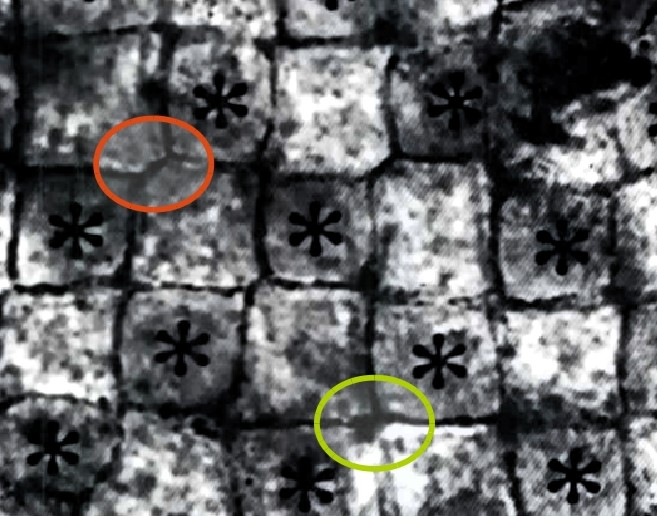
\includegraphics[width=0.5\textwidth]{../diagrams/checkers.jpg}
\caption[Square Cells.]{An image or Japanese quail epithelium. This tissue is patterned like a checkerboard and has been modeled in the past as a tissue with degree three vertices. It is possible that modelling this tissue as degree four vertices would provide better approximations of the dynamics.  In particular, notice that the orange vertices clearly can be modeled with degree three, wherease the green vertex could be one degree four vertex or two degree three.\cite{Checkers}}
\end{figure}


\section{Feedback Mechanisms and Proliferation}
This model is limited in that includes neither mechanical nor chemical feedback, and does not specify how cells proliferate. These are two extensions which can and have been made to the model by certain researchers. On the other hand, the dynamics of some successful models such as \cite{Morphogen} have the patterning of cells specified entirely by morphogens. In these models, chemicals called `morphogens' are what drive cells to proliferate, and the low concentrations of the morphogen on the fringe of the tissue explain why the tissue eventually ceases to grow as the tissue reaches a certain size.  Other models, such as those described in \cite{MechanicalFeedback} are based upon the vertex dynamics models such as the Honda-Nagai model, but include additional mechanical feedback terms which limit the growth of cells. 

\section{Additional Curiosities}
The vast majority of models assume that exactly three cells meet at any  vertex, except vertices on the boundary. In the language of topology, one would  say that all interior vertices in the tissue have degree three. Empirical observations show, however, that more more than three cells can meet at any junction under certain circumstances \cite{Vertex Models}. This means that models ought to be extended to include the formation of these `rosettes'.

